%\section{Preliminaries}
\label{sec:prelims}

\newcommand{\vm}{\mathrm{V}\MemModel}

A program can be associated with a set of `execution graphs'\cite{lahavveri}, each of which represents a possible run of the program and captures the accesses to shared variables (events), together with the relationships between these accesses. The consistency of each  execution graph is then determined by the rules associated with a memory model.
We shall now define execution graphs and some auxiliary  relations required to check their consistency.

%Unlike SC, where consistency is checked via an interleaving, release-acquire semantics requires reasoning with two special types of relations on the reads and writes: a reads-from relation $\rf$ (mapping each read to the write it observes) and a per-location modification order $\mo$ (ordering writes to the same variable). The verification question becomes: does there exist $\rf$ and $\mo$ on the observed events that satisfy the axioms for the release-acquire memory model? The presentation in this section follows~\cite{Lahav:2022,ChakrabortyKMP24} and introduces these preliminaries.


\noindent \textbf{Events.} An \emph{event} is a memory operation: either a read $\rd(x, v)$ or write $\wt(x, v)$, where $x \in \varset$ is a shared memory location  and $v \in \valset$ is a value that is either read-from or written-to the memory location. These are the analogues of ``$read(x,v)$'' and ``$write(x,v)$'' that were used in~\cite{gibbons} and recalled in the prelimaniries of Part A. We sometimes use the term \emph{variable} for a memory location. For an event $e$, we write $e.\op$, $e.\lloc$ and $e.\val$ respectively for the memory operation ($\rd$ or $\wt$), the shared memory location and the value associated with the event. We sometimes write $\rd(x)$ in short for a read event $\rd(x, v)$ when the value $v$ is not important to the context. Similarly, we write $\wt(x)$ for a write event $\wt(x, v)$. When the variable $x$ is also clear from the context, we simply write $\rd, \wt$ for $\rd(x), \wt(x)$.

Events are spread across a set of \emph{threads}.
For a set of events $\E$, we write $\E.\R$ and $\E.\W$ for the set of all read and write events in $\E$ respectively, and $\E.\R_x, \E.\W_x$ for the read and write events involving variable $x$. When the set of events $\E$ is clear from the context, we simply write $\R_x$ and $\W_x$. 

\noindent \textbf{Execution graph.} An \emph{execution graph} ~\cite{Lahav:2017} (also known as candidate execution~\cite{Batty:2011}) is a tuple $\ex = \tup{\E, \po, \rf, \mo}$  where $\E$ is a set of events and $\po$, $\rf$, $\mo$ are binary relations over $\E$. 
The \emph{program order} $\po$ is a partial order that enforces a total order on events of the same thread. 
The \emph{reads-from relation} $\rf\subseteq (\E.\W \times \E.\R)$ associates write
 events $\event_1$ to read events $\event_2$. It can be seen as an edge $e_1 \xra{~\rf~} e_2$ from (the node corresponding to) $e_1$ to (the node corresponding to) $e_2$ in the execution graph $\ex$. 
Indeed, it must be that $\event_1.\lloc=\event_2.\lloc$, $\event_1.\val=  \event_2.\val$ and every read event has a unique writer ($\rfinv$ is a function). 
The \emph{modification order} $\mo\subseteq (\E.\W\times \E.\W)$ is the union of modification orders $\mo_x$ for $x \in \varset$, where each $\mo_x$ is a total order over the set $\locx{\W}$ of write events that involve variable $x$. For a read $r$, let $\rf^{-1}(r)$ denote the write associated by $\rf$ to $r$, in other words, it is the write from which $r$ reads from according to $\rf$.

A \emph{partial execution graph} $\expartial=\tup{\E, \po}$ is an abstraction of execution graphs which does not contain the modification order and the reads-from relation.

\noindent \textbf{Consistency.} Consistency of an observed execution graph with respect to a weak memory model can be characterized using certain properties of the combination consisting of the $\po$, $\rf$ and $\mo$ relations -- these properties are called \emph{consistency axioms}. In Section~\ref{subsec:consistency_axioms}, we formally define the consistency axioms of release-acquire memory model ($\ramm$) and its close variants strong release-acquire ($\sramm$) and weak release-acquire ($\wramm$) and $\rlxmm$. 

\noindent{\bf{Notations for Relations}}. 
Let $S$ be a binary relation over the set of events $\E$.  The reflexive, transitive, reflexive-transitive closures, and inverse relations of $S$ 
are denoted as $S^?$, $S^+$, $S^*$, $S^{-1}$ respectively. 
The relation $S$ is \emph{acyclic} if $S^+$ is irreflexive. 
We write $\irr(S)$ and $\acy(S)$ to denote that  relation $S$ is irreflexive and acyclic respectively.  The identity relation on a set $B$ is denoted as $[B]$ : 
$[B](x,y) \triangleq x = y \land x \in B$.
The composition of two relations $S_1$ and $S_2$, is denoted by $S_1;S_2$. 
For a shared variable $x$, we let $S_x=[\locx{\E}];S;[\locx{\E}]$ be the restriction of $S$ to all events of $\E$ on $x$, with $\locx{\E} = \{ e \in E \mid e.\var = x \}$.

\noindent \textbf{Derived relations.} The \emph{from-read relation} $\fr \subseteq \R \times \W$ relates every read event to all the write events that are $\mo$-after its own write (olive coloured dotted edges in Figure~\ref{examplesra}(d) are $\fr$ relations). The $\fr$ edge explicitly denotes that in any interleaving with $\wt~\rf~\rd$ and $\wt~\mo~\wt'$ $\wt'$ should be ordered after $\rd$.

The \emph{happens-before relation} $\hb$ is the transitive closure of $\po$ and $\rf$. In our descriptions, we view $\hb$ as a path consisting of $\xra{\po}$ and $\xra{\rf}$ edges.

%Happens-before ($\hb$) where all the $\rf$ edges are projected to an individual variable $x$ is denoted as  $\hb_x$.
 %More precisely: 
 %$\hb \triangleq (\po\cup \rf)^+$, and $\hb_x \triangleq (\po\cup \rf_x)^+$.

 
 \subsection{Consistency Axioms}\label{subsec:consistency_axioms}
The axioms are broadly classified as  
\emph{coherence} and \emph{causality cycles}. We will describe them in detail below. Table~\ref{table:ax:models-2} summarizes the list of axioms and indicates the axioms for each memory model, and Figure~\ref{fig:illust} gives scenarios violating the various axioms.



\noindent{\bf{Coherence}}. The modification order $\mo$ enforces an `SC-per-variable' constraint in any execution $\ex$, that is, memory accesses per shared variable are  totally ordered.  Coherence axioms essentially describe rules on this modification order  $\mo$.
 
\emph{Write-coherence} enforces that $\mo$ agrees with $\hb$ for each variable (denoted as $\irr(\mo_x;\hb)$ in Table~\ref{table:ax:models-2} and a violation of it is shown in Figure~\ref{fig:illust}(b)): intuitively, if a write $\wt(x, v_1)$ happens-before $\wt(x, v_2)$, then $x$ is updated to $v_1$ first, and then $v_2$. As the order of updates to $x$ is encoded by the modification order $\mo_x$, the axiom requires $\mo_x$ to align with $\hb$.  
A stronger version of it, called \emph{strong-write-coherence}, requires the entire $\mo$ (and not just $\mo_x$) to align with $\hb$, in other words, it requires the acyclicity of $\po \cup \rf \cup \mo$ -- again, notice that this requirement is across variables, as $\mo=\bigcup_{x \in \varset}\mo_x$. Execution graph in Figure~\ref{fig:illust}(e) violates strong-write-coherence, while it does not violate write-coherence. A weakened form of write-coherence is
relaxed-write-coherence, where $\hb$ is simply $\po$. Figure~\ref{fig:illust}(g) shows a violation of \RlxWCoh{}.

 \emph{Read coherence}  enforces that a read $\rd(x)$ cannot read from a write $\wt_1(x)$ if 
there is an \emph{intermediate} write $\wt_2(x)$ that happens-before $\rd(x)$, 
i.e. $(\wt_2(x), \rd(x)) \in \hb$ (denoted as $\wt_2(x) \xra{\hb} \rd(x)$), and ``intermediate'' refers to $\mo$,
i.e.,  $(\wt_1(x),\wt_2(x))\in \mo$ (denoted as $\wt_1(x) \xra{\mo} \wt_2(x)$). Said differently, if $\wt_1(x)$ and $\wt_2(x)$ happen-before a read $\rd(x)$, then $\wt_1(x) \xra{\mo} \wt_2(x)$, implies $\rd(x)$ cannot read from $\wt_1(x)$. The $\mo$ relation makes $\wt_1$ stale for $\rd$. Figure~\ref{fig:illust}(c) shows a violation of read-coherence. 
In a weaker form of read-coherence called
\emph{weak-read-coherence}~\cite{Lahav:2022} (Figure~\ref{fig:illust}(d)), 
``intermediate'' relates to $\hb$ (and not $\mo$), i.e., we have $\wt_1(x) \xra{\hb} \wt_2(x)$: in other words, if $\wt_1(x) \xra{\hb} \wt_2(x) \xra{\hb} \rd(x)$, then $\rd$ cannot read from $\wt_1$. Figure~\ref{fig:illust}(f) demonstrates violation of another form of weakening called \emph{relaxed-read-coherence} which involves replacing $\hb$ with just $\po$.
 
\noindent{\bf{Causality cycles}}. A causality cycle consists of $\po$ and $\rf$ orderings.
The C11 models explicitly mandate \PORF{} \cite{Lahav:2022,Luo:2021}, that is, 
$\acy(\po \cup \rf)$ (Figure~\ref{fig:illust}(a)). 

\begin{table*}
  \vspace{-\baselineskip}
  %\caption{Global caption}
  \begin{minipage}{.45\linewidth}
    \caption{\small Coherence Axioms for C11 variants}
    \label{table:ax:models-1}
    %\centering
    \scalebox{0.8}{
    %\small
    \begin{tabular}{lr}
    \multicolumn{2}{c|}{\underline{Release-Acquire}} \\
    $\irr(\mo_x;\hb)$ & (\WCoh{})\\
    $\acy(\hb \cup \mo)$ & (\SWCoh{})\\
    $\irr(\rf^{-1};\mo_x;\hb)$ & (\RCoh{})\\
    $\irr(\hb_x;[\W];\hb;\rf^{-1})$ & (\WRCoh{})\\
    \hline
    \multicolumn{2}{c}{\underline{Relaxed}} \\
    $\irr(\mo_x;\po)$ & (\RlxWCoh{})\\
    $\irr(\rf^{-1};\mo_x;\rf^?;\po)$ & (\RlxRCoh{})\\
    \end{tabular}
    }
    \end{minipage}%
    \hspace{0.1in}
  \begin{minipage}{.45\linewidth}
    %\centering
      \caption{\small The C11 models $\wramm, \ramm, \sramm, \rlxmm$.}
      \label{table:ax:models-2}
      \scalebox{0.7}{
        \setlength\tabcolsep{7.5pt}
      \begin{tabular}{lr|lr}
      \multicolumn{2}{l|}{} & \multicolumn{2}{l}{} \\
      $\wramm$ & \makecell{\PORF{}\\ \WRCoh{}} &$\rlxmm$ & \makecell{\PORF{}\\ \RlxRCoh\\ \RlxWCoh} \\ 
      \hline
      $\ramm$ & \makecell{\PORF{} \\
      \WCoh{}\\ \RCoh{}}   &$\sramm$ & \makecell{\PORF{}\\ \SWCoh{}\\ \RCoh{}}\\ 
      \cline{1-4}
      %$\sramm$ & \makecell{\SWCoh{}\\ \RCoh{}} & & \\ 
      \end{tabular}
      }        
      \end{minipage} 
%      \vspace{-\baselineskip}
  \end{table*}

\iffalse
\begin{table}[t!]
     \caption{\small Models $\wramm, \ramm, \sramm$.}
    \label{table:ax:models-2}  
        \setlength\tabcolsep{7.5pt}
      \begin{tabular}{lr|lr}
      \multicolumn{2}{l|}{} & \multicolumn{2}{l}{} \\
       &  & $\irr(\mo_x;\hb)$  (\WCoh{})~~ & \\
     $\wramm$ & \makecell{\PORF{}\\ \WRCoh{}} &$\irr(\rf^{-1};\mo_x;\hb)$  (\RCoh{})&\\  
      &&$\acy(\hb \cup \mo)$  (\SWCoh{})~~& \\
       && $\irr(\hb;[\W_x];\hb;\rf^{-1}_x)~~~$ (\WRCoh{})& \\
      \hline
      $\ramm$ & \makecell{\PORF{} \\
      \WCoh{}\\ \RCoh{}}   &$\sramm$  \makecell{\PORF{}\\ \SWCoh{}\\ \RCoh{}} &\\ 
      \cline{1-4}
      \end{tabular}
          
  \end{table}
\fi


\begin{figure*}[t]
    \def\ystep{0.4}
     \resizebox{\textwidth}{!}{
	\begin{tikzpicture}[yscale=1]
        \node (t11) at (0,0*\ystep)  {$\rd(x)$};
      \node (t12) at (0,-4*\ystep) {$\wt(y)$};
    %
      \node (t21) at (1.8,0,0*\ystep) {$\rd(y)$};
      \node (t22) at (1.8,-4*\ystep) {$\wt(x)$};
     \node (t23) at (1,-4.9*\ystep) {$(a)$};
    
      \draw[po] (t11) to (t12);
    %  
      \draw[po] (t21) to (t22);
    %
      \draw[rf,bend left=0] (t12) to node[above,pos=0.1, sloped]{$\rf$} (t21);
      \draw[rf,bend right=0] (t22) to node[above,pos=0.1, sloped]{$\rf$} (t11);
    %%%%%%%%%%%%%%%%%%%%%%%%%%%%%%%%%%%%%%%%%%%%%%%%%%%%%%%%%
      
      
      \node (t11) at (2.9,0*\ystep)  {$\wt_1(x)$};
      \node (t12) at (2.9,-4*\ystep) {$\wt(y)$};
    %
      \node (t21) at (4.7,0*\ystep) {$\rd(y)$};
      \node (t22) at (4.7,-4*\ystep) {$\wt_2(x)$};
    %  \node (t23) at (1.8,-4.5*\ystep) {$\rd(x)$};
    %
     \node (t23) at (3.9,-4.9*\ystep) {$(b)$};
    
      \draw[po] (t11) to (t12);
    %  
      \draw[po] (t21) to (t22);
    %   \draw[po] (t22) to (t23);
    %
      \draw[rf,bend left=0] (t12) to node[above,pos=0.9, sloped]{$\rf$} (t21);
    %  \draw[rf,bend left=0] (t11) to node[below,pos=0.9, sloped]{$\rf$} (t23);
    %    
      \draw[mo,bend left=0] (t22) to node[above,pos=0.8, sloped]{$\mo$} (t11);
    
    %%%%%%%%%%%%%%%%%%%%%%%%%%%%%%%%%%%%%%%%%%%%%%%%%%%%
      \node (t11) at (6,0*\ystep)  {$\wt_1(x)$};
      \node (t12) at (6,-2*\ystep) {$\wt_2(x)$};
      \node (t13) at (6,-4*\ystep) {$\wt(y)$};
    %
      \node (t21) at (7.8,0*\ystep) {$\rd(y)$};
      \node (t22) at (7.8,-4*\ystep) {$\rd(x)$};
     \node (t23) at (7,-4.9*\ystep) {$(c)$};
    
    %  \draw[po] (t11) to (t12);
      \draw[po] (t12) to (t13);
    %
      \draw[po] (t21) to (t22);
    %
     \draw[mo] (t11) to node[left]{$\mo$} (t12);
    %
      \draw[rf,bend left=0] (t13) to node[above,pos=0.8, sloped]{$\rf$} (t21);
      \draw[rf,bend left=5] (t11) to node[above,pos=0.8, sloped]{$\rf$} (t22);
    %    
    %  \draw[fr,bend right=0] (t22) to node[below,pos=0.2, sloped]{$\fr$} (t12);
    %%%%%%%%%%%%%%%%%%%%%%%%%%%%%%%%%%%%%%%%%%%%%%%%%%%%%%%%%%%%%%%%%%%%%%%%%%%%%%%
      \node (t11) at (9.1,0*\ystep)  {$\wt_1(x)$};
      \node (t12) at (9.1,-4*\ystep) {$\wt(y)$};
    %
      \node (t21) at (10.9,0*\ystep) {$\rd(y)$};
      \node (t22) at (10.9,-2*\ystep) {$\wt_2(x)$};
      \node (t23) at (10.9,-4*\ystep) {$\rd(x)$};
    \node (t24) at (10,-4.9*\ystep) {$(d)$};
      \draw[po] (t11) to (t12);
    %  
      \draw[po] (t21) to (t22);
      \draw[po] (t22) to (t23);
    %
      \draw[rf,bend left=0] (t12) to node[above,pos=0.8, sloped]{$\rf$} (t21);
      \draw[rf,bend right=0] (t11) to node[below,pos=0.8, sloped]{$\rf$} (t23);
    
    %%%%%%%%%%%%%%%%%%%%%%%%%%%%%%%%%%%%%%%%%%%%%%%%%%%%%%%%%%%%%%%%%%%%%%%%%%%%%%%%%%
     \node (t11) at (12.2,0*\ystep)  {$\wt(y)$};
      \node (t12) at (12.2,-4*\ystep) {$\wt(x)$};
    %  \node (t13) at (0,-4.5*\ystep) {$\rd(x)$};
    %
      \node (t21) at (14,0*\ystep) {$\wt(x)$};
      \node (t22) at (14,-4*\ystep) {$\wt(y)$};
      \node (t23) at (13.1,-4.9*\ystep) {$(e)$};
    %
      \draw[po] (t11) to (t12);
    %  \draw[po] (t12) to (t13);
    %  
      \draw[po] (t21) to (t22);
    %  \draw[po] (t22) to (t23);
    %
    %  \draw[rf,bend left=0] (t11) to node[below,pos=0.9, sloped]{$\rf$} (t23);
    %  \draw[rf,bend right=0] (t21) to node[below,pos=0.9, sloped]{$\rf$} (t13);
    %    
      \draw[mo,bend left=0] (t12) to (t21);
      \draw[mo,bend right=0] (t22) to node[above,pos=0.8, sloped]{$\mo$} (t11);
    %%%%%%%%%%%%%%%%%%%%%%%%%%%%%%%%%%%%%%%%%%%%%%%%%%%%%%%%%%%%%%%%%%%%%%%%%%%%%%%%%
     \node (t11) at (15.3,0*\ystep)  {$\wt_1(x)$};
      \node (t12) at (15.3,-4*\ystep) {$\wt_2(x)$};
    %  \node (t13) at (0,-4.5*\ystep) {$\rd(x)$};
    %
      \node (t21) at (17.1,0*\ystep) {$\rd_2(x)$};
      \node (t22) at (17.1,-4*\ystep) {$\rd_1(x)$};
      \node (t23) at (16.2,-4.9*\ystep) {$(f)$};
    %
      \draw[mo] (t11) to node[left]{$\mo$} (t12);
    %  \draw[po] (t12) to (t13);
    %  
      \draw[po] (t21) to (t22);
    %  \draw[po] (t22) to (t23);
    %
    %  \draw[rf,bend left=0] (t11) to node[below,pos=0.9, sloped]{$\rf$} (t23);
    %  \draw[rf,bend right=0] (t21) to node[below,pos=0.9, sloped]{$\rf$} (t13);
    %    
      \draw[rf,bend left=0] (t12) to node[above, pos=.8, sloped]{$\rf$}(t21);
      \draw[rf,bend right=0] (t11) to node[below,pos=0.8, sloped]{$\rf$} (t22);
      
      %%%%%%%%%%%%%%%
      %%%%%%%%%%%%%%%
      
      \node (t11) at (18.4,0*\ystep)  {$\wt_1(x)$};
      
      \node (t12) at (18.4,-4*\ystep) {$\wt_1(x)$};
      
      \draw[mo,bend left=30] (t12) to node[left]{$\mo$} (t11);
    %  \draw[po] (t12) to (t13);
    %  
      \draw[po] (t11) to (t12);
      
      \node (t23) at (18.4,-5*\ystep) {$(g)$};
    %
    \end{tikzpicture}
	 }
    \caption{\footnotesize (a)\PORF{} is violated (b)\WCoh{} is violated: $\wt_1(x)~\hb~\wt_2(x)$ while 
    $\wt_2(x)~\mo~\wt_1(x)$, 
     (c)\RCoh{} is violated: $\wt_1(x)~\rf~\rd(x)$ with $\wt_1(x)~\mo~\wt_2(x)$ and $\wt_2(x)~\hb~\rd(x)$, 
       (d)\WRCoh{} is violated: $\wt_1(x)~\rf~\rd(x)$ with $\wt_1(x)~\hb~\wt_2(x)$
      and $\wt_2(x)~\hb~\rd(x)$,    (e)\SWCoh{} is violated : $\hb \cup \mo$ cycle, (f)\RlxRCoh{} is violated: $\wt_1(x)~\mo~\wt_2(x)$, $\rd_2(x)~\po~\rd_1(x)$ 
      with $\wt_2(x)~\rf~\rd_2(x)$ and $\wt_1(x)~\rf~\rd_1(x)$, (g)\RlxWCoh{} is violated}
      \label{fig:illust}
\end{figure*}

We now demonstrate the precise set of consistency axioms for all C11 memory models including $\scmm$. Figure~\ref{examplesra} shows illustrations to distingush the relevant memory models.

\paragraph*{Sequential Consistency} This is stronger than coherence, which orders only
accesses on the same shared variable. An execution graph is $\scmm$ iff it violates $\acy(\po\cup\rf\cup\mo\cup\fr)$.       

\paragraph*{Release-Acquire and variants} In all variants of $\ramm$, synhronization is obtained via $\rf$ and the happens before relation is $\hb \triangleq (\po\cup \rf)^+$. Follwing \cite{Lahav2021} we study three variants of release-acquire: $\ramm$, $\sramm$, $\wramm$. While $\sramm$ has strong-write-coherence guarantees, $\wramm$ does not place any restrictions on the $\mo$ ordering between same-location writes. Instead, the only orderings considered between same-location writes are through the $[\W];\hb_{x};[\W]$ relation, $x\in\varset$. Thus, $\wramm$ provides weaker constraints for coherence and atomicity.

\paragraph*{Relaxed} The relaxed memory model has the least synchronization mechanism amongst all C11 variants. Here, $\hb = \po$ while applying the coherence axioms.


\begin{figure*}[h]
%  \vspace{-\baselineskip}
  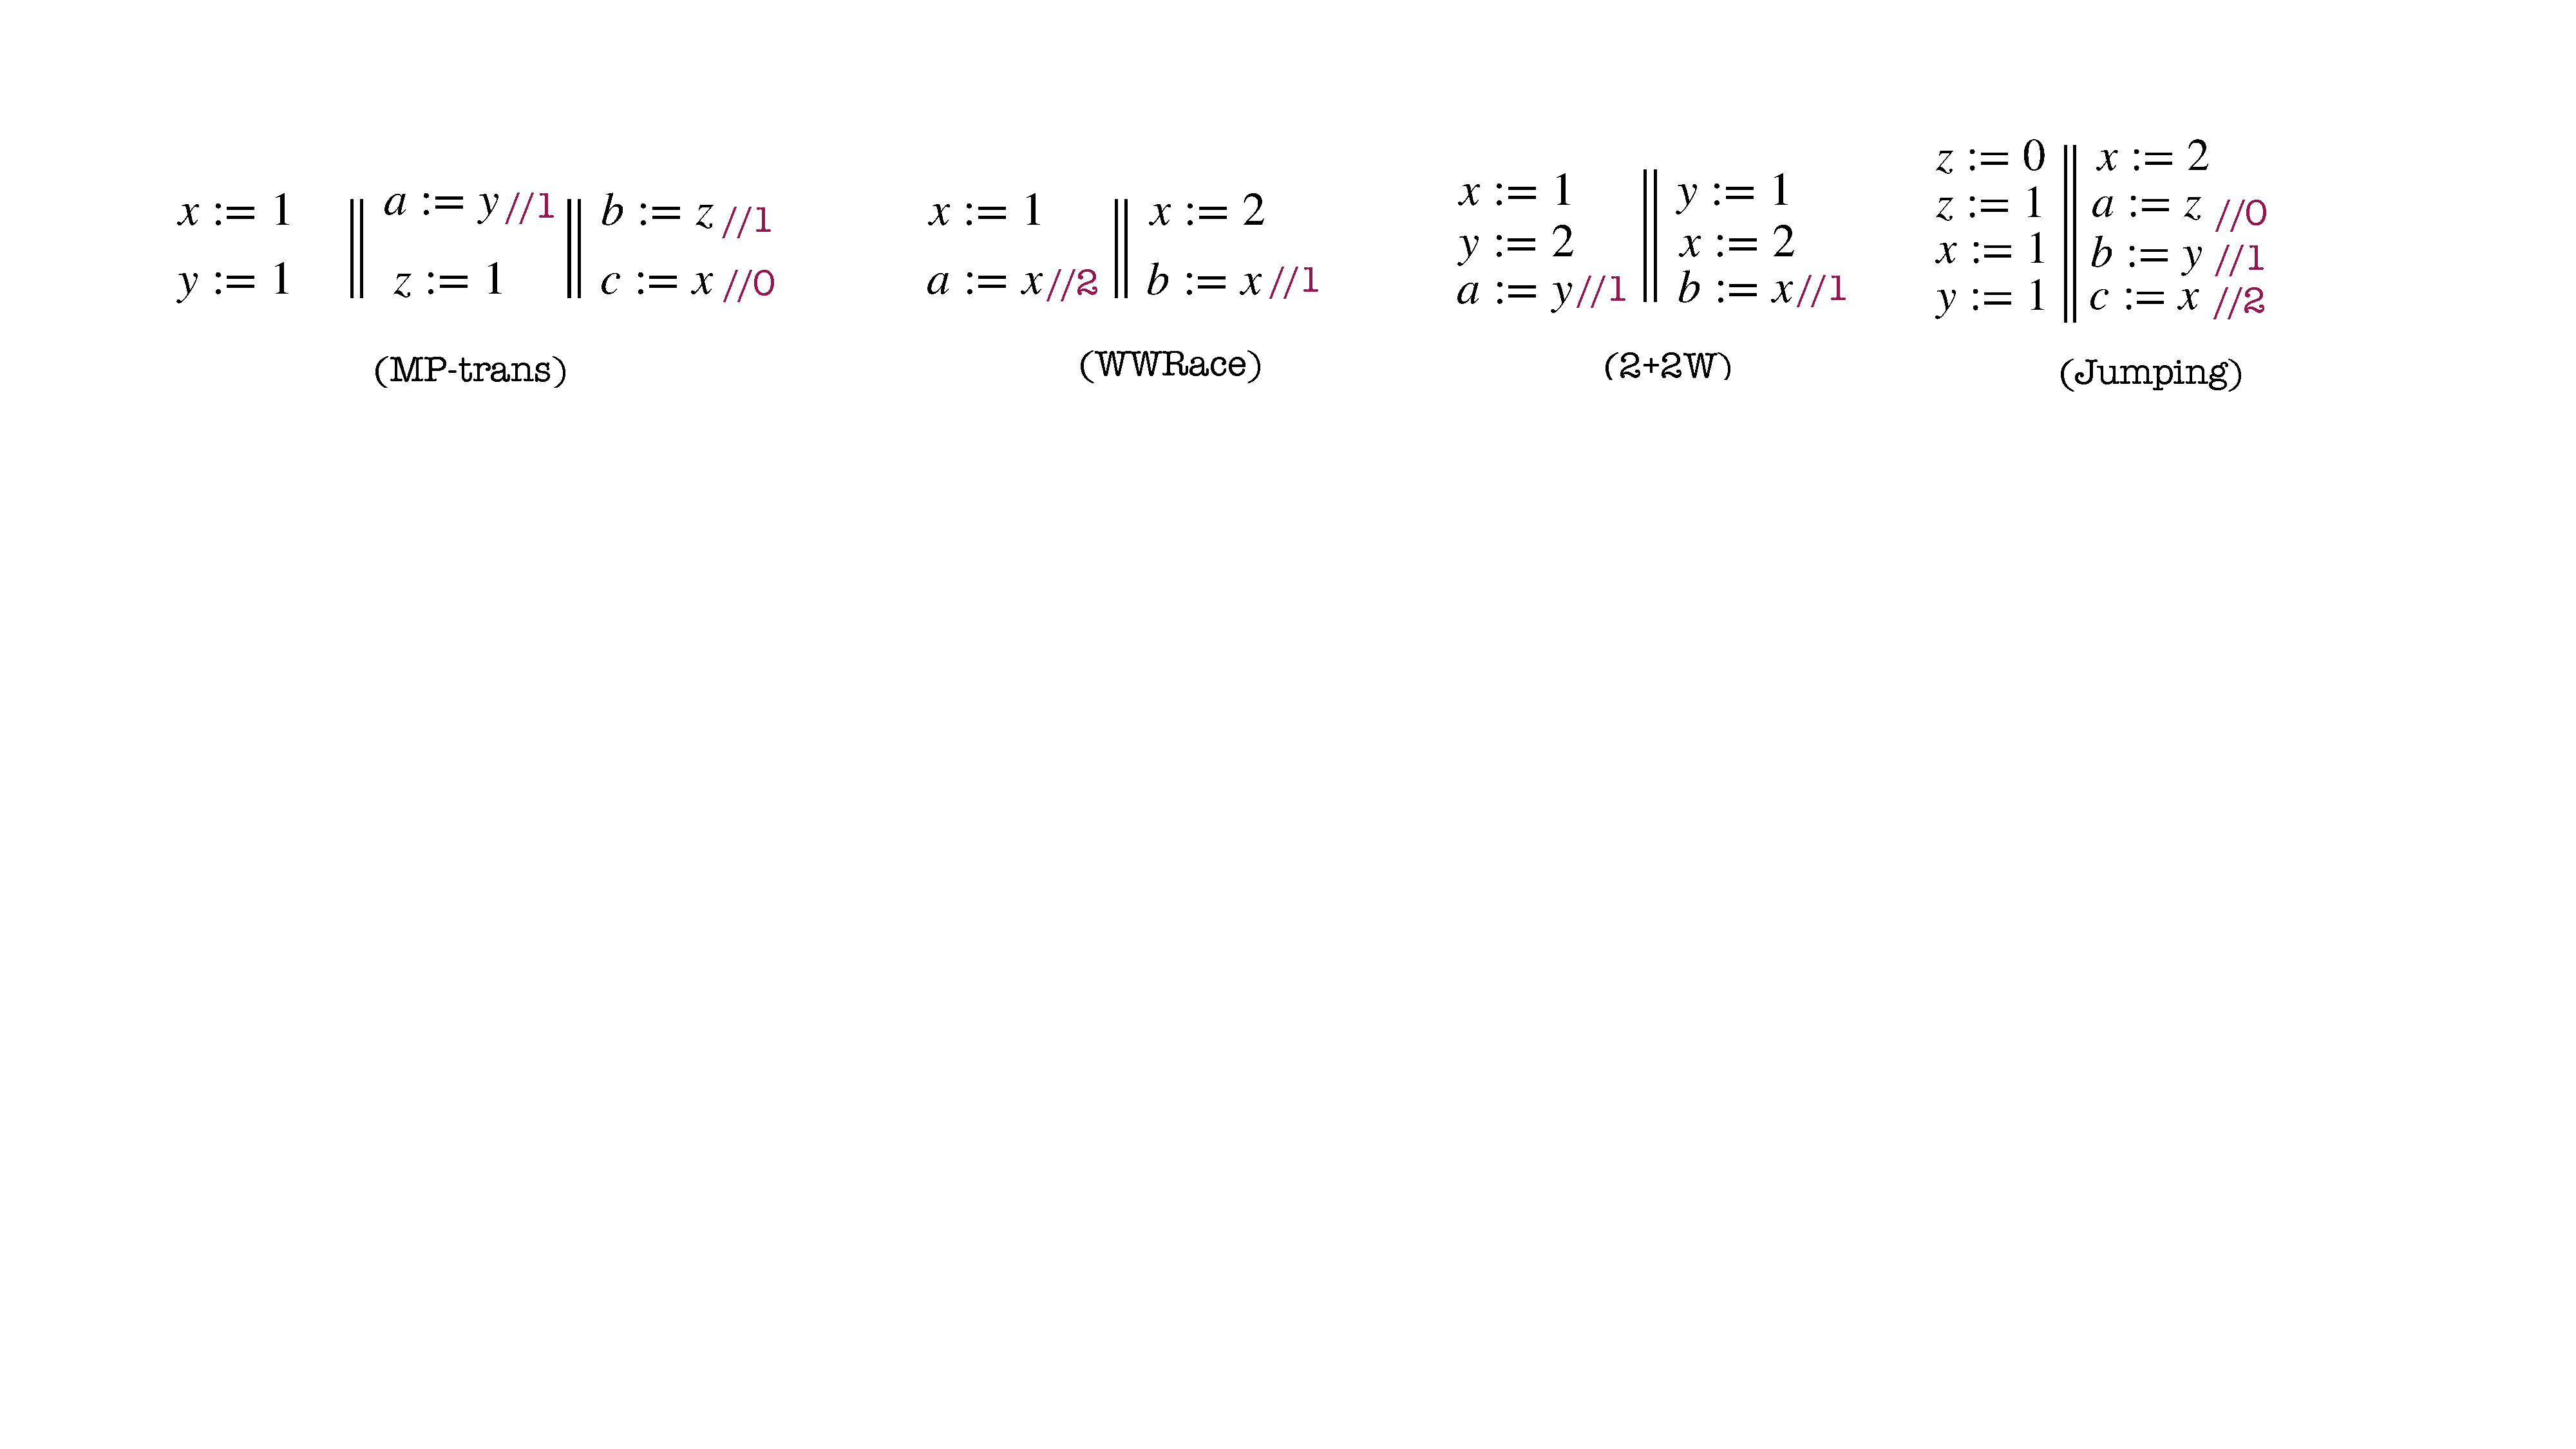
\includegraphics[width=\textwidth]{examples-violation.pdf}
%\vspace{.5cm}
\def\ystep{0.4}
 \begin{tikzpicture}[yscale=1.2]
 \begin{scope}[scale=.9]
  
 

    \node (t11) at (0,0*\ystep)  {\textcolor{green!30!blue}{$\wt(x,0)$}};
      \node (t12) at (1.5,0*\ystep) {\textcolor{green!30!blue}{$\wt(y,0)$}};
\node (t13) at (3.3,0*\ystep) {\textcolor{green!30!blue}{$\wt(z,0)$}};
    
    
    \node (t21) at (-.2,-4*\ystep)  {$\wt(x,1)$};
      \node (t22) at (1.5,-4*\ystep) {$\rd(y,1)$};
\node (t23) at (3.5,-4*\ystep) {$\rd(z,1)$};
    
   
   \node (t31) at (-.2,-8*\ystep)  {$\wt(y,1)$};
      \node (t32) at (1.5,-8*\ystep) {$\wt(z,1)$};
\node (t33) at (3.5,-8*\ystep) {$\rd(x,0)$};
\node (t34) at (2,-9.3*\ystep) {$(a)$};
    
    

  \draw[po] (t11) to (t21);
  
  \draw[po] (t12) to (t22);
  
\draw[po] (t13) to (t23);


  \draw[po] (t21) to (t31);
  
  \draw[po] (t22) to (t32);
  
\draw[po] (t23) to (t33);


  \draw[rf,bend right=-10] (t11) to node[above,pos=.5, sloped]{$\rf$} (t33);
  
  \draw[rf,bend right=20] (t32) to node[above,pos=0.8, sloped]{$\rf$} (t23);
  
  \draw[rf,bend right=20] (t31) to node[above,pos=0.8, sloped]{$\rf$} (t22);
  
%%%%%%%%%%%%%%%%%%%%%%%%%%%%%%%%%%%%%%%%%%%%%%%%%%%%%%%%%%%%%%%%%%%%%%%%%%%%%%%%%%%%%%%
%\node (t11) at (6.5,0*\ystep)  {$\wt(x,0)$};
     
    
    \node (t21) at (5.5,-4*\ystep)  {$\wt(x,1)$};
      \node (t22) at (5.5,-8*\ystep) {$\rd(x,2)$};
      
\node (t31) at (7.5,-4*\ystep)  {$\wt(x,2)$};
      \node (t32) at (7.5,-8*\ystep) {$\rd(x,1)$};

 %\draw[po] (t11) to (t21);
%\draw[po] (t11) to (t31);


  \draw[rf,bend right=0] (t31) to node[above,pos=.7, sloped]{$\rf$} (t22);
\draw[rf,bend right=0] (t21) to node[above,pos=.7, sloped]{$\rf$} (t32);

  \draw[mo,bend right=-30] (t21) to node[above,pos=.5, sloped]{$\mo$} (t31);
\draw[mo,bend right=-20] (t31) to node[below,pos=.5, sloped]{$\mo$} (t21);

\node (t33) at (6.5,-9.3*\ystep) {$(b)$};
 \draw[po] (t21) to (t22);
  
  \draw[po] (t31) to (t32);
 
%%%%%%%%%%%%%%%%%%%%%%%%%%%%%%%%%%%%%%%%%%%%%%%%%%%%%%%%%%%%%%%%%%%%%%%%%%%%%%%%%%%%%    
%\node (t11) at (9.5,0*\ystep)  {\textcolor{green!30!blue}{$\wt(x,0)$}};
%\node (t12) at (11.5,0*\ystep)  {\textcolor{green!30!blue}{$\wt(y,0)$}};
     
    \node (t21) at (9.5,-2.5*\ystep)  {$\wt(x,1)$};
      \node (t22) at (9.5,-5*\ystep) {$\wt(y,2)$};
            \node (t23) at (9.5,-7.5*\ystep) {$\rd(y,1)$};


    \node (t31) at (11.5,-2.5*\ystep)  {$\wt(y,1)$};
      \node (t32) at (11.5,-5*\ystep) {$\wt(x,2)$};
            \node (t33) at (11.5,-7.5*\ystep) {$\rd(x,1)$};
\node (t34) at (10.5,-9.3*\ystep) {$(c)$};

% \draw[po] (t11) to (t21);
\draw[po] (t21) to (t22);
\draw[po] (t22) to (t23);

% \draw[po] (t12) to (t31);
\draw[po] (t31) to (t32);
\draw[po] (t32) to (t33);
     
     
  \draw[rf,bend right=0] (t31) to node[above,pos=.9, sloped]{$\rf$} (t23);
\draw[rf,bend right=0] (t21) to node[below,pos=.7, sloped]{$\rf$} (t33);

  \draw[mo,bend right=0] (t22) to (t31);
\draw[mo,bend right=0] (t32) to node[above,pos=.5]{$\mo$} (t21);
%%%%%%%%%%%%%%%%%%%%%%%%%%%%%%%%%%%%%%%%%%%%%%%%%%%%%%%%%%%%%%%%%%%%%%%%%%%%%%%%%%%%%%

    \node (t20) at (13.5,0*\ystep)  {$\wt(z,0)$};

     
    \node (t21) at (13.5,-2.5*\ystep)  {$\wt(z,1)$};
      \node (t22) at (13.5,-5*\ystep) {$\wt(x,1)$};
            \node (t23) at (13.5,-7.5*\ystep) {$\wt(y,1)$};

    \node (t30) at (15.5,0*\ystep)  {$\wt(x,2)$};
    \node (t31) at (15.5,-2.5*\ystep)  {$\rd(z,0)$};
      \node (t32) at (15.5,-5*\ystep) {$\rd(y,1)$};
            \node (t33) at (15.5,-7.5*\ystep) {$\rd(x,2)$};
\node (t34) at (14.5,-9.3*\ystep) {$(d)$};

\draw[po] (t20) to (t21);
\draw[po] (t21) to (t22);
\draw[po] (t22) to (t23);

 \draw[po] (t30) to (t31);
\draw[po] (t31) to (t32);
\draw[po] (t32) to (t33);
     
     
  \draw[rf,bend right=0] (t20) to node[above,pos=.9, sloped]{$\rf$} (t31);
\draw[rf,bend right=0] (t23) to node[above,pos=.7, sloped]{$\rf$} (t32);
\draw[rf,bend right=-40] (t30) to node[below,pos=.7, sloped]{$\rf$} (t33);
    

  \draw[fr,bend right=-10] (t31) to node[above,pos=.5]{$\fr$}(t21);
  \draw[fr,bend right=-10] (t33) to node[below,pos=.5]{$\fr$}(t22);
  
\draw[mo,bend left=-40] (t20) to node[left,pos=.7]{$\mo$} (t21);
\draw[mo,bend left=10] (t30) to node[below,pos=.7]{$\mo$} (t22);
\end{scope}
\vspace{-\baselineskip}

   \end{tikzpicture}
\caption{\footnotesize(a) execution graph of MP-trans violating $\wramm$ : we have  $\wt(x,0)~\hb~\wt(x,1)~\hb~\rd(x,0)~\rf^{-1}~\wt(x,0)$ which violates weak-read-coherence. (b) execution graph of WWrace consistent with $\wramm$ but violating $\ramm$ : we have $\rd(x,1)~\rf^{-1}\wt(x,1)~\mo~\wt(x,2)~\hb~\rd(x,1)$ violating read coherence. (c) execution graph of 2+2W which is $\ramm$ consistent but violating 
$\sramm$ : we have $\wt(x,1)~\hb~\wt(y,2)~\mo~\wt(y,1)~\hb~\wt(x,2)~\mo~\wt(x,1)$ violating strong-write-coherence. (d) 
execution graph of Jumping which is $\sramm$ consistent, but violates $\scmm$: we have $\wt(x,1)~\po~\wt(y,1)~\rf~\rd(y,1)~\po~\rd(x,2)~\fr~\wt(x,1)$ violating 
$\acy(\po \cup \rf \cup \mo \cup \fr)$.
 }
\label{examplesra}
\vspace{-\baselineskip}
\end{figure*}


Here are a couple of useful lemmas describing the relationship between the three models $\ramm$, $\sramm$, $\wramm$ and $\rlxmm$.
 
\begin{lemma}\label{lem:sra-ra-wra-relationship}
Let $\ex = \tuple{\E, \po, \rf, \mo}$ be an execution graph. Then: $\ex \models \sramm$ implies $\ex \models \ramm$, and $\ex \models \ramm$ implies $\ex \models \wramm$. 
\end{lemma} 
\begin{proof}
  It is easy to see that if $\ex$ satisfies strong-write-coherence, then it satisfies write-coherence also. Hence $\ex \models \sramm$ implies $\ex \models \ramm$. For $\ramm$ to $\wramm$, we show that if weak-read-coherence is violated, then either read-coherence or write-coherence is violated: suppose weak-read-coherence is violated, there is a cycle $\rd(x) \xra{\rf^{-1}} \wt_1(x) \xra{\hb} \wt_2(x) \xra{\hb} \rd(x)$. The $\mo$ relation can order $\wt_1$ and $\wt_2$ in either way. If $\wt_1(x) \xra{\mo} \wt_2(x)$, then read-coherence is violated, and if $\wt_2(x) \xra{\mo} \wt_2(x)$, then write-coherence is violated.
\end{proof}

\begin{lemma}\label{lem:sra-ra-rlx-relationship}
Let $\ex = \tuple{\E, \po, \rf, \mo}$ be an execution graph. Then: $\ex \models \ramm$ implies $\ex \models \rlxmm$, and $\ex \models \ramm$ implies $\ex \models \rlxmm$. 
\end{lemma}

\begin{proof}

If $\ex$ satisfies \WCoh{}, then it satisfies \RlxWCoh. Similarly, if $\ex$ satisfies \RCoh{}, then $\ex$ also satisfies \RlxRCoh{}. This is because in both cases $\hb$ is replaced by $\po$ in the coherence axioms. Hence $\ex \models \ramm$ implies $\ex \models \rlxmm$.

\end{proof}

 
\begin{figure*}[h]
%  \vspace{-\baselineskip}
%\vspace{.5cm}
\begin{center}
 

\def\ystep{0.4}
 \begin{tikzpicture}[yscale=1.2]
 \begin{scope}[scale=1]
 %wra
    \node (t21) at (0,0*\ystep)  {$\wt(x,1)$};
      \node (t22) at (0,-3*\ystep) {$\rd(x,2)$};
     \node (t31) at (2,0*\ystep) {$\wt(x,2)$};
     \node (t32) at (2,-3*\ystep) {$\rd(x,1)$};

\node (t34) at (1,-4*\ystep) {$(a)$};

% \draw[po] (t11) to (t21);
\draw[po] (t21) to (t22);
\draw[po] (t31) to (t32);
 
     
  \draw[rf,bend right=0] (t21) to node[above,pos=.9, sloped]{$\rf$} (t32);
\draw[rf,bend right=0] (t31) to node[below,pos=.7, sloped]{$\rf$} (t22);

  \draw[mo,bend right=5] (t21) to (t31);
\draw[mo,bend right=5] (t31) to node[above,pos=.5]{$\mo$} (t21);
%%%%%%%%%%%%%%%%%%%%%%%%%%%%%%%%%%%%%%%%%%%%%%%%%%%%%%%%%%%%%%%%%%%%%%%%%%%%%%%%%%%%%%

%%rlx
\node (t21) at (6,0*\ystep)  {$\wt(x,1)$};
      \node (t22) at (6,-3*\ystep) {$\wt(x,2)$};
      \node (t23) at (6,-6*\ystep) {$\wt(y,1)$};
      
     \node (t31) at (8,0*\ystep) {$\rd(y,1)$};
     \node (t32) at (8,-6*\ystep) {$\rd(x,1)$};

\node (t34) at (7,-7*\ystep) {$(b)$};

% \draw[po] (t11) to (t21);
\draw[po] (t21) to (t22);
\draw[po] (t22) to (t23);
\draw[po] (t31) to (t32);
 
     
  \draw[rf,bend right=0] (t23) to node[above,pos=.7, sloped]{$\rf$} (t31);
\draw[rf,bend right=0] (t21) to node[below,pos=.7, sloped]{$\rf$} (t32);
 \end{scope}
\vspace{-\baselineskip}


   \end{tikzpicture}
   \end{center}
\caption{\footnotesize (a) $\wramm$-consitent but violates \RlxRCoh{} and hence not $\rlxmm$-consistent.
 (b) $\rlxmm$-consitent but violates \WRCoh{} and hence not $\wramm$-consistent.
 }\label{example-rlxwra}
\vspace{-\baselineskip}
\end{figure*}
\paragraph*{Comparing memory models.} The two lemmas gives the following partial order of the memory models reflecting the number of allowed behaviours: $\scmm\preccurlyeq\sramm\preccurlyeq\ramm\preccurlyeq\{\wramm,\rlxmm\}$ with models towards the right allowing more behaviors.  All models are weaker than $\scmm$. $\rlxmm$ is weaker than $\ramm$ but incomparable with $\wramm$. In particular, the lack of synchronization across $\rf$
in $\rlxmm$ makes $\hb$ weaker in $\rlxmm$ compared to $\wramm$. On the other hand, $\wramm$ allows extra behaviors over $\rlxmm$ because it does not enforce \WRCoh{}. Figure~\ref{example-rlxwra} shows examples to demonstrate the incomparability between $\wramm$ and $\rlxmm$.

An execution graph $\ex = \tuple{\E, \po, \rf, \mo}$ is consistent with memory model $\MemModel$ if it satisfies all the axioms corresponding to $\MemModel$ as shown in Table  ~\ref{table:ax:models-2}. We write $\ex \models \MemModel$ if $\ex$ is consistent with $\MemModel$. For a partial execution graph $\expartial = \tuple{\E, \po}$, we write $\expartial \models \MemModel$ if there exists an $\rf$ and $\mo$ such that $\ex \models \MemModel$ for the complete execution graph $\ex = \tuple{\E, \po, \rf, \mo}$. Hence, the general consistency testing problem $\vm$ can be stated as: given a partial execution graph $\expartial$ and a memory model $\MemModel$, does $\expartial \models \MemModel$? 
Alternatively, we can frame the problem as follows.
\begin{center}
  \fbox{%
    \begin{minipage}{0.98\textwidth}
      \noindent \textsc{Verifying weak memory consistency} (The $\vm$-problem)

      \medskip

      \noindent \textbf{Instance:} A partial execution graph $\expartial=\tuple{\E, \po}$ and a memory model $\MemModel \in \{\ramm, \sramm, \wramm, \rlxmm\}$

      \medskip

      \noindent \textbf{Question:} Do there exist $\rf$ and $\mo$ relations on $\E$ such that the complete execution graph $\ex = \tuple{\E, \po, \rf, \mo}$ satisfies the consistency axioms of the memory model $\MemModel$?
    \end{minipage}%
  }
\end{center}

The next chapter shall solely deal with the above problem. We shall, as in VSC$^\pp$, classify the results based on the number of writers per variable. The next two chapters would contain relevant theorems and proofs related for $\vm$ when the model is $\ramm$. The weak and strong variants of $\ramm$ are also placed alongside in these chapters.

The following two chapters will be dedicated to results related to $\rlxmm$ memory model and even later we shall discuss similar results for  some of the causal memory models. I have not left any detailing about them here. We shall understand them as they appear.






